\documentclass[10pt,letterpaper]{article}
\usepackage[english]{babel}
\usepackage{graphicx}
\usepackage[margin=2cm]{geometry}

\usepackage{amsfonts}
\usepackage{amsmath}
\usepackage{amsthm}
\newcommand{\dif}[1][]{\mathrm{d} {#1}\,}
\newcommand{\rb}[1]{ \left(  {#1} \right) }
\newcommand{\frb}[1]{ \left(  {#1} \right) }

\usepackage{float}
\usepackage{subcaption}

% \usepackage[amsmath,thmmarks,standard]{ntheorem}
\newtheoremstyle{break}
{\topsep}
{\topsep}%
{\normalfont}
{}%
{\bfseries}
{}%
{\newline}
{}%
\theoremstyle{break}
\newtheorem{exercise}{Exercise}
\newtheorem*{information}{Information}
\newtheorem{solution}{Solution}
\newtheorem*{solutioninformation}{Solution Information}




% \usepackage{amsmath}
% \usepackage{mathtools}
% %\usepackage[a4paper]{geometry}
% %\usepackage{amsfonts}
% \usepackage{amssymb}
% \usepackage{amsthm}
% \usepackage{mathrsfs}
% \usepackage{bm}
% \usepackage{algpseudocode}
% \usepackage{upgreek}
% \usepackage{subcaption}


\usepackage{graphicx}
\usepackage{epstopdf}

% \mathtoolsset{showonlyrefs}

%\usepackage{epstopdf}
\usepackage{graphicx} 

%\usepackage[pdf]{pstricks}

% \usepackage[shortlabels]{enumitem}
% %Standard operator
% \newcommand{\abs}[1]{\lvert #1\rvert}
% \newcommand{\supp}{Peratorname{supp}}
% \newcommand{\grad}{{\mathbf{grad}}}
% \newcommand{\curl}{\normalfont{\text{curl}}}
% \newcommand{\Log}{\text{Log}}
% \newcommand{\cc}{{\normalfont{\text{c}}}}
% \newcommand{\loc}{{\normalfont{\text{loc}}}}

% \DeclareMathOperator*{\argmax}{arg\,max}
% \DeclareMathOperator*{\argmin}{arg\,min}

% % Package for colors
% \usepackage{xcolor}
% \definecolor{ao}{rgb}{0.0, 0.5, 0.0}

% %Edit colors







%\usepackage{fancyhdr}
%\usepackage{datetime}
%
%\fancyhf{}
%\fancyfoot[L]{\fontsize{10}{12} \today \ \currenttime}
%\pagestyle{fancy} \usepackage{tikz}

% \DeclareSymbolFont{extraup}{U}{zavm}{m}{n}
% \DeclareMathSymbol{\varheart}{\mathalpha}{extraup}{86}
% \DeclareMathSymbol{\vardiamond}{\mathalpha}{extraup}{87}

% \usepackage{chngcntr}
% \counterwithout{equation}{subsection}
% \counterwithout{equation}{section} 

\usepackage{tikz}

\newcommand\encircle[1]{%
  \tikz[baseline=(X.base)] 
    \node (X) [draw, shape=circle, inner sep=0] {\strut #1};}





\begin{document}


\title{Characteristics and Weak solutions}
\date{}

\maketitle 

















\begin{exercise}[Entropy Solutions]
	Consider the conservation law 
	\begin{align}
		\frac{\partial u}{\partial t}
		+
		\frac{\partial f(u)}{\partial x}
		= 0,
		\quad
		u(x,0)=u_0(x),
	\end{align}
	and $f(u) = u^2/2$.
	Consider the following initial conditions
	\begin{align}
		\text{(a)}
		\,\,\;\;
		u_0(x) = 
		\left\{
		\begin{array}{cl}
		1, & \text{for} \quad x<-1,\\
		0, &\text{for} \quad -1<x< 1,\\
		-1, &\text{for} \quad x > 1
		\end{array}
		\right.
		\quad
		\text{and}
		\quad
		\text{(b)}
		\,\,\;\;
		u_0(x) = 
		\left\{
		\begin{array}{cl}
		-1, & \text{for} \quad x<-1,\\
		0, &\text{for} \quad -1<x < 1, \\
		1, &\text{for} \quad x > 1.
		\end{array}
		\right.
	\end{align}
	Draw the profile of $u_0(x)$ and sketch the characteristics
	of the entropy solution $u(x,t)$ in the $x-t$ plane, and
	determine $u(x,t)$ for all $t > 0$.
\end{exercise}

\begin{solution}
	We start with the solution driven by the initial data
	\begin{equation}\label{InCond1}
		u_{0}(x)
		=
		\begin{cases}
			1 & x<-1\\
			0 & -1<x<1\\
			-1 & x>1
		\end{cases}\ .
	\end{equation}
	Figure 1 contains a sketch of the initial data profile
	$u_{0}\!\left(x\right)$ with characteristics evolving.
	We see that two discontinuities are present in the initial data.
	The task is to determine the exact solution $u\!\left(x,t\right)$ for all $t>0$.
	For Burger's equation, a shock forms if $u_{l}>u_{r}$.
	Thus, both discontinuities in the initial function produce shocks.
	To determine the speed of each shock we use the Rankine-Hugoniot 
	jump condition
	\begin{equation}
		s=\frac{f({u_{l}})-f({u_{r}})}{u_{l}-u_{r}}\ .
	\end{equation}
	Applied to each discontinuity in the initial data, we get
	\begin{equation}
		s_{1}=\frac{\frac{1}{2}1^{2}-\frac{1}{2}0^{2}}{1-0}=\frac{1}{2}
		\qquad\qquad
		s_{2}=\frac{\frac{1}{2}0^{2}-\frac{1}{2}\left(-1\right)^{2}}{0-\left(-1\right)}=-\frac{1}{2}\ .
	\end{equation}
	The left shock moves to the right and the right shock moves to the left.
	From this we expect the two shocks to meet at $x=0$ at time $t=2$.
	We can now write the exact solution up until $t=2$: 
	\begin{equation}
		u\!\left(x,t\right)
		=
		\begin{cases}
			1 & x<\frac{1}{2} t-1\\
			0 & \frac{1}{2} t-1<x<-\frac{1}{2}t +1\\
			-1 & -\frac{1}{2} t +1<x
		\end{cases}\ .
	\end{equation}
	When the two shocks meet we are left with a Riemann problem.
	This time, the ``initial condition'' is the solution we have calculated at $t=2$.
	Again we turn to the Rankine-Hugoniot jump condition. This time, the shock's speed is
	\begin{equation}
		s_{3}=\frac{\frac{1}{2}1^{2}-\frac{1}{2}\left(-1\right)^{2}}{1-\left(-1\right)}=0\ .
	\end{equation}
	When the two shocks meet they stop moving for all time hereafter.
	Thus, for $t>2$, 
	\begin{equation}
		u(x,t)
		=
		\begin{cases}
			1 & x<0\\
			-1 & 0<x
		\end{cases}\ .
	\end{equation}

	Now we move on to the solution for the initial data set
	\begin{equation}\label{InCond2}
		u_{0}(x)
		=
		\begin{cases}
			-1 & x<-1\\
			0 & -1<x<1\\
			1 & 1<x
		\end{cases}\ .
	\end{equation}
	In Figure 2 is a sketch of the initial data profile
	$u_{0}(x)$ with characteristics evolving
	as rarefaction waves.
	A general solution model for a rarefaction wave on
	a Riemann problem is supplied in the exercise
	description for initial data centered at zero.
	Using the solution model with 
	$f'\!\left(v\left(\xi\right)\right)=\xi\Rightarrow v\!\left(\xi\right)=\xi$ we arrive at
	\begin{equation}
		u(x,t)
		=
		\begin{cases}
			-1 & x<-t-1\\
			\frac{x+1}{t} & -t-1<x<-1\\
			0 & -1<x<1 \\
			\frac{x-1}{t} & 1<x<t+1\\
			1 & t+1<x
		\end{cases}\ .
	\end{equation}

	\usetikzlibrary{arrows}
\begin{tikzpicture}[scale=2,pile/.style={thick, ->, >=stealth', shorten <=2pt, shorten >=2pt}]

	%\draw[very thick] plot coordinates{ (-1.75,1) (-1,1) (-1,0) (1,0) (1,-1) (1.75,-1) }; 
	\draw (1.25,0.7) node { $\,$ };
												
\end{tikzpicture}
%
%\draw plot coordinates{point sequence};	
%\draw plot ;	
%	\draw[smooth] plot coordinates{(0,0),{};
% \draw [smooth,very thick] (0,0) -- (4,-3) -- (8,-5) -- (12,-6);
% \draw[smooth,domain=0:6.5] plot function{sin(2*x)*exp(-x/4)};
% \draw[ycomb,color=gray,line width=0.5cm] plot coordinates{(1,1) (2,2) (3,3)};

	\begin{figure}[H]
	\center 

	\subfloat[\label{fig:Exc1_3a_U}]{\usetikzlibrary{arrows}
\begin{tikzpicture}[scale=2.1,pile/.style={thick, ->, >=stealth', shorten <=2pt, shorten >=2pt}]

	\draw[very thick] plot coordinates{ (-1.75,1) (-1,1) (-1,0) (1,0) (1,-1) (1.75,-1) }; 
	\draw [-] (-1.75,0) -- (1.75,0);
	\draw [dashed] (-1,1) -- (-0.4,1);
	\draw [dashed] (-0.4,1) -- (-0.4,0);
	\draw [dashed] (1,-1) -- (0.4,-1);
	\draw [dashed] (0.4,-1) -- (0.4,0);
	
	\draw [->,thick] (-0.9,0.5) -- (-0.5,0.5);	
	\draw [->,thick] (0.9,-0.5) -- (0.5,-0.5);	
	
	\draw [->,thick] (-1.5,-0.7) -- (-1.5,-0.5);	
	\draw [->,thick] (-1.5,-0.7) -- (-1.3,-0.7);	
	
	\draw (-1.6,-0.6) node { $u$ };
	\draw (-1.4,-0.8) node { $x$ };

	\draw[ ] plot coordinates{ (0,0.1) (0,-0.1) };	
	\draw (0,-0.3) node { $0$ };
	%\draw (1.25,0.7) node { $u_0(x)$ };

	% Draw fourth fine propagation  
	%\fill[gray!30] (12.5,-3) -- (14,-3) -- (14,-2) -- (12.5,-2) -- (12.5,-3);

	% Draw grid
	%\draw[] plot coordinates{ (0,0) (0,-5) (14,-5) };  
	
	
	
	%\draw [->,very thick] (0,-5.75) -- (2,-5.75);		
	%\draw (1,-5.4) node { $Time$ };

	%\draw [<->,dashed,thick ] (0,1.5) -- (3,1.5);
	%\draw[thick] plot coordinates{ (3,1.4) (3,1.6) };
	
	%\draw (1.5,2) node {$Iter.\,k=0$};	
		
    % Labels
	%\draw (-1.5,0.5) node {$Proc.\,1$};

	% Draw first coarse propagation
	%\fill[gray!90] (0,0) -- (0,1) -- (0.5,1) -- (0.5,0) -- (0,0);
	%\draw[] plot coordinates{ (0,0) (0,1) (0.5,1) (0.5,0) (0,0) };  

	%\draw (13.25,-4.5) node {{\scriptsize $T_{\mathcal{G}}$}};
													
\end{tikzpicture}
%
%\draw plot coordinates{point sequence};	
%\draw plot ;	
%	\draw[smooth] plot coordinates{(0,0),{};
% \draw [smooth,very thick] (0,0) -- (4,-3) -- (8,-5) -- (12,-6);
% \draw[smooth,domain=0:6.5] plot function{sin(2*x)*exp(-x/4)};
% \draw[ycomb,color=gray,line width=0.5cm] plot coordinates{(1,1) (2,2) (3,3)};


	}\hspace{10mm}\subfloat[\label{fig:Exc1_3a_C}]{\usetikzlibrary{arrows}
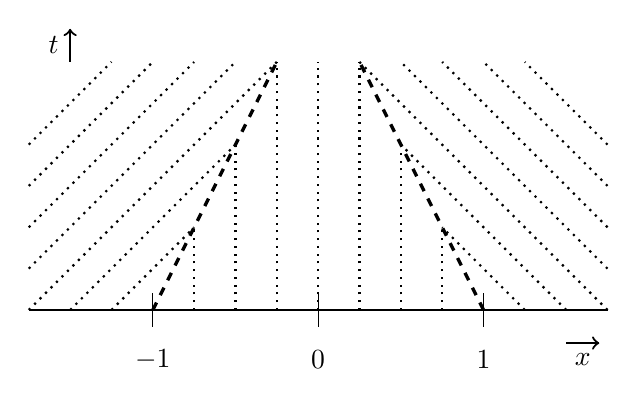
\begin{tikzpicture}[scale=2.1,pile/.style={thick, ->, >=stealth', shorten <=2pt, shorten >=2pt}]

	% Axes
	\draw [-] (-1.75,0) -- (1.75,0);
	\draw[] plot coordinates{ (-1,0.1) (-1,-0.1) };	
	\draw[] plot coordinates{ (0,0.1) (0,-0.1) };	
	\draw[] plot coordinates{ (1,0.1) (1,-0.1) };	
	\draw (-1,-0.3) node { $-1$ };
	\draw (0,-0.3) node { $0$ };
	\draw (1,-0.3) node { $1$ };
	\draw [->,thick] (1.5,-0.2) -- (1.7,-0.2);	
	\draw [->,thick] (-1.5,1.5) -- (-1.5,1.7);		
	\draw (1.6,-0.3) node { $x$ };
	\draw (-1.6,1.6) node { $t$ };

	% Shocks
	\draw [dashed,very thick] (-1,0) -- (-0.25,1.5);
	\draw [dashed,very thick] (1,0) -- (0.25,1.5);
	
	% Straight
	\draw [dotted,thick] (-0.75,0) -- (-0.75,0.5);
	\draw [dotted,thick] (-0.50,0) -- (-0.50,1);
	\draw [dotted,thick] (-0.25,0) -- (-0.25,1.5);
	\draw [dotted,thick] (0,0) -- (0,1.5);
	\draw [dotted,thick] (0.25,0) -- (0.25,1.5);
	\draw [dotted,thick] (0.50,0) -- (0.50,1);
	\draw [dotted,thick] (0.75,0) -- (0.75,0.5);

	% Slopes left
	\draw [dotted,thick] (-1.25,0) -- (-0.75,0.5);
	\draw [dotted,thick] (-1.50,0) -- (-0.50,1);		
	\draw [dotted,thick] (-1.75,0) -- (-0.25,1.5);	
	\draw [dotted,thick] (-1.75,0.25) -- (-0.5,1.5);		
	\draw [dotted,thick] (-1.75,0.50) -- (-0.75,1.5);	
	\draw [dotted,thick] (-1.75,0.75) -- (-1.00,1.5);	
	\draw [dotted,thick] (-1.75,1.00) -- (-1.25,1.5);	
	
	% Slopes right
	\draw [dotted,thick] (1.25,0) -- (0.75,0.5);
	\draw [dotted,thick] (1.50,0) -- (0.50,1);		
	\draw [dotted,thick] (1.75,0) -- (0.25,1.5);	
	\draw [dotted,thick] (1.75,0.25) -- (0.5,1.5);		
	\draw [dotted,thick] (1.75,0.50) -- (0.75,1.5);	
	\draw [dotted,thick] (1.75,0.75) -- (1.00,1.5);	
	\draw [dotted,thick] (1.75,1.00) -- (1.25,1.5);	
			
													
\end{tikzpicture}

	}

	\caption{\label{fig:Exc1_3a} Exercise 3.1a. Initial data $u_0$ given by \label{InCond1}, applied to the inviscid burgers equation. The two shocks move towards each other and merge at $x=0$. At $x=0$ they form a new stationary shock.
	\quad{(a)}~ Initial data. \quad{(b)}~Characteristics. }

	\end{figure}

	\begin{figure}[H] 
	\center 

	\subfloat[\label{fig:Exc1_3b_U}]{\usetikzlibrary{arrows}
\begin{tikzpicture}[scale=2.1,pile/.style={thick, ->, >=stealth', shorten <=2pt, shorten >=2pt}]

	\draw[very thick] plot coordinates{ (-1.75,-1) (-1,-1) (-1,0) (1,0) (1,1) (1.75,1) }; 
	\draw [-] (-1.75,0) -- (1.75,0);
	\draw [dashed] (-1,0) -- (-1.6,-1);
	\draw [dashed] (1,0) -- (1.6,1);
	
	\draw [->,thick] (-1.1,-0.8) -- (-1.4,-0.8);	
	\draw [->,thick] (1.1,0.8) -- (1.4,0.8);	
	
	\draw [->,thick] (-1.5,0.5) -- (-1.5,0.7);	
	\draw [->,thick] (-1.5,0.5) -- (-1.3,0.5);	
	
	\draw (-1.6,0.6) node { $u$ };
	\draw (-1.4,0.4) node { $x$ };
	%\draw (1.25,0.7) node { $u_0(x)$ };

	\draw[ ] plot coordinates{ (0,0.1) (0,-0.1) };	
	\draw (0,-0.3) node { $0$ };


	% Draw fourth fine propagation  
	%\fill[gray!30] (12.5,-3) -- (14,-3) -- (14,-2) -- (12.5,-2) -- (12.5,-3);

	% Draw grid
	%\draw[] plot coordinates{ (0,0) (0,-5) (14,-5) };  
	
	
	
	%\draw [->,very thick] (0,-5.75) -- (2,-5.75);		
	%\draw (1,-5.4) node { $Time$ };

	%\draw [<->,dashed,thick ] (0,1.5) -- (3,1.5);
	%\draw[thick] plot coordinates{ (3,1.4) (3,1.6) };
	
	%\draw (1.5,2) node {$Iter.\,k=0$};	
		
    % Labels
	%\draw (-1.5,0.5) node {$Proc.\,1$};

	% Draw first coarse propagation
	%\fill[gray!90] (0,0) -- (0,1) -- (0.5,1) -- (0.5,0) -- (0,0);
	%\draw[] plot coordinates{ (0,0) (0,1) (0.5,1) (0.5,0) (0,0) };  

	%\draw (13.25,-4.5) node {{\scriptsize $T_{\mathcal{G}}$}};
													
\end{tikzpicture}
%
%\draw plot coordinates{point sequence};	
%\draw plot ;	
%	\draw[smooth] plot coordinates{(0,0),{};
% \draw [smooth,very thick] (0,0) -- (4,-3) -- (8,-5) -- (12,-6);
% \draw[smooth,domain=0:6.5] plot function{sin(2*x)*exp(-x/4)};
% \draw[ycomb,color=gray,line width=0.5cm] plot coordinates{(1,1) (2,2) (3,3)};


	}\hspace{10mm}\subfloat[\label{fig:Exc1_3b_C}]{\usetikzlibrary{arrows}
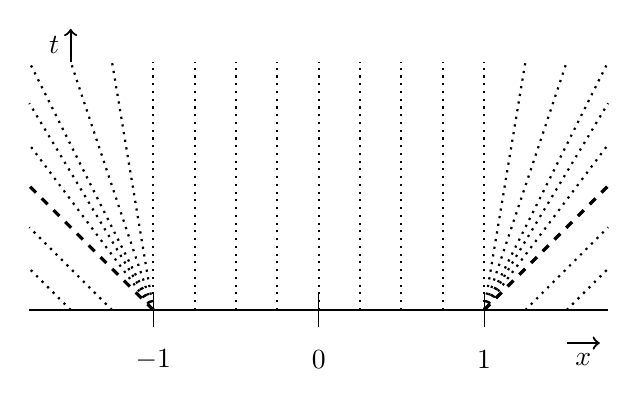
\begin{tikzpicture}[scale=2.1,pile/.style={thick, ->, >=stealth', shorten <=2pt, shorten >=2pt}]

	% Axes
	\draw [-] (-1.75,0) -- (1.75,0);
	\draw[] plot coordinates{ (-1,0.1) (-1,-0.1) };	
	\draw[] plot coordinates{ (0,0.1) (0,-0.1) };	
	\draw[] plot coordinates{ (1,0.1) (1,-0.1) };	
	\draw (-1,-0.3) node { $-1$ };
	\draw (0,-0.3) node { $0$ };
	\draw (1,-0.3) node { $1$ };
	\draw [->,thick] (1.5,-0.2) -- (1.7,-0.2);	
	\draw [->,thick] (-1.5,1.5) -- (-1.5,1.7);		
	\draw (1.6,-0.3) node { $x$ };
	\draw (-1.6,1.6) node { $t$ };
	
	% Straight
	\draw [dotted,thick] (-1,0) -- (-1,1.5);
	\draw [dotted,thick] (-0.75,0) -- (-0.75,1.5);
	\draw [dotted,thick] (-0.5,0) -- (-0.5,1.5);
	\draw [dotted,thick] (-0.25,0) -- (-0.25,1.5);
	\draw [dotted,thick] (0,0) -- (0,1.5);
	\draw [dotted,thick] (0.25,0) -- (0.25,1.5);
	\draw [dotted,thick] (0.5,0) -- (0.5,1.5);	
	\draw [dotted,thick] (0.75,0) -- (0.75,1.5);	
	\draw [dotted,thick] (1,0) -- (1,1.5);


	% Slopes left
	\draw [dotted,thick] (-1.5,0) -- (-1.75,0.25);
	\draw [dotted,thick] (-1.25,0) -- (-1.75,0.50);
	\draw [dashed, very thick] (-1,0) -- (-1.75,0.75);
	\draw [dotted,thick] (-1,0) -- (-1.75,1);
	\draw [dotted,thick] (-1,0) -- (-1.75,1.25);
	\draw [dotted,thick] (-1,0) -- (-1.75,1.50);
	\draw [dotted,thick] (-1,0) -- (-1.50,1.50);
	\draw [dotted,thick] (-1,0) -- (-1.25,1.50);
				
	% Slopes right
	\draw [dotted,thick] (1.5,0) -- (1.75,0.25);
	\draw [dotted,thick] (1.25,0) -- (1.75,0.50);
	\draw [dashed,very thick] (1,0) -- (1.75,0.75);
	\draw [dotted,thick] (1,0) -- (1.75,1);
	\draw [dotted,thick] (1,0) -- (1.75,1.25);
	\draw [dotted,thick] (1,0) -- (1.75,1.50);
	\draw [dotted,thick] (1,0) -- (1.50,1.50);
	\draw [dotted,thick] (1,0) -- (1.25,1.50);			
													
\end{tikzpicture}


	}

	\caption{\label{fig:Exc1_3b} Exercise 3.1b. Initial data $u_0$, given by \label{InCond2}, applied to the inviscid burgers equation. The two rarefaction waves move away from each other with equal speed and never merge. \quad{(a)} Initial data. \quad{(b)} Characteristics. }

	\end{figure}

	\begin{figure}[H]
	\center 

	\subfloat[\label{fig:Exc1_4_U}]{\usetikzlibrary{arrows}
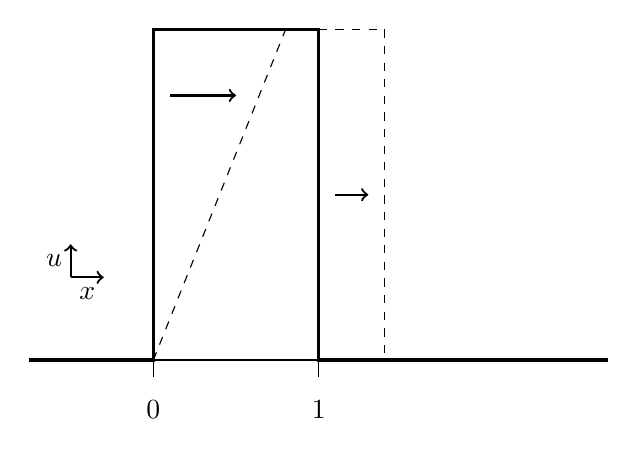
\begin{tikzpicture}[scale=2.1,pile/.style={thick, ->, >=stealth', shorten <=2pt, shorten >=2pt}]

	\draw[very thick] plot coordinates{ (-0.75,0) (0,0) (0,2) (1,2) (1,0) (2.75,0) }; 
	\draw [-] (-0.75,0) -- (2.75,0);
	\draw [dashed] (0,0) -- (0.8,2);
	\draw [dashed] (0.8,2) -- (1.4,2);
	\draw [dashed] (1.4,2) -- (1.4,0);
	
	\draw [->,thick] (-0.5,0.5) -- (-0.5,0.7);	
	\draw [->,thick] (-0.5,0.5) -- (-0.3,0.5);	

	
	\draw [->,thick] (0.1,1.6) -- (0.5,1.6);		
	\draw [->,thick] (1.1,1) -- (1.3,1);	
	
	\draw (-0.6,0.6) node { $u$ };
	\draw (-0.4,0.4) node { $x$ };

	\draw[] plot coordinates{ (0,0.1) (0,-0.1) };	
	\draw[] plot coordinates{ (1,0.1) (1,-0.1) };	
	\draw (0,-0.3) node { $0$ };
	\draw (1,-0.3) node { $1$ };

	%\draw (2.25,0.7) node { $u_0(x)$ };

	% Draw fourth fine propagation  
	%\fill[gray!30] (12.5,-3) -- (14,-3) -- (14,-2) -- (12.5,-2) -- (12.5,-3);

	% Draw grid
	%\draw[] plot coordinates{ (0,0) (0,-5) (14,-5) };  
	
	
	
	%\draw [->,very thick] (0,-5.75) -- (2,-5.75);		
	%\draw (1,-5.4) node { $Time$ };

	%\draw [<->,dashed,thick ] (0,1.5) -- (3,1.5);
	%\draw[thick] plot coordinates{ (3,1.4) (3,1.6) };
	
	%\draw (1.5,2) node {$Iter.\,k=0$};	
		
    % Labels
	%\draw (-1.5,0.5) node {$Proc.\,1$};

	% Draw first coarse propagation
	%\fill[gray!90] (0,0) -- (0,1) -- (0.5,1) -- (0.5,0) -- (0,0);
	%\draw[] plot coordinates{ (0,0) (0,1) (0.5,1) (0.5,0) (0,0) };  

	%\draw (13.25,-4.5) node {{\scriptsize $T_{\mathcal{G}}$}};
													
\end{tikzpicture}
%
%\draw plot coordinates{point sequence};	
%\draw plot ;	
%	\draw[smooth] plot coordinates{(0,0),{};
% \draw [smooth,very thick] (0,0) -- (4,-3) -- (8,-5) -- (12,-6);
% \draw[smooth,domain=0:6.5] plot function{sin(2*x)*exp(-x/4)};
% \draw[ycomb,color=gray,line width=0.5cm] plot coordinates{(1,1) (2,2) (3,3)};


	}\hspace{10mm}\subfloat[\label{fig:Exc1_4_C}]{\usetikzlibrary{arrows}
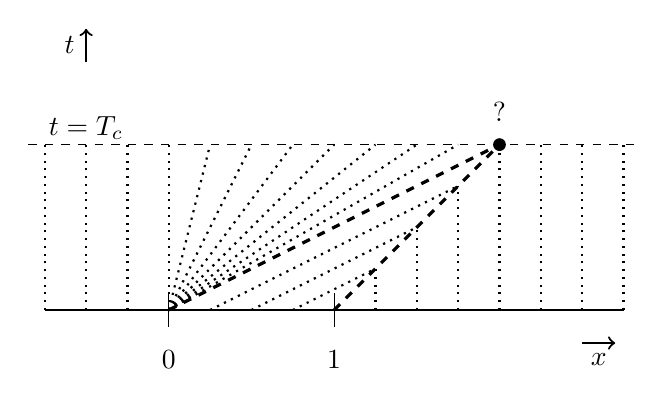
\begin{tikzpicture}[scale=2.1,pile/.style={thick, ->, >=stealth', shorten <=2pt, shorten >=2pt}]

	\draw [-] (-0.75,0) -- (2.75,0);
	\draw [dashed, very thick] (1,0) -- (2,1);
	

	% Straight
	\draw [dotted,thick] (-0.75,0) -- (-0.75,1.00);
	\draw [dotted,thick] (-0.50,0) -- (-0.50,1.00);
	\draw [dotted,thick] (-0.25,0) -- (-0.25,1.00);
	\draw [dotted,thick] (-0.0,0) -- (-0.0,1.00);		
	\draw [dotted,thick] (1.25,0) -- (1.25,0.25);
	\draw [dotted,thick] (1.50,0) -- (1.50,0.50);
	\draw [dotted,thick] (1.75,0) -- (1.75,0.75);
	\draw [dotted,thick] (2.00,0) -- (2.00,1.00);	
	\draw [dotted,thick] (2.25,0) -- (2.25,1.00);	
	\draw [dotted,thick] (2.50,0) -- (2.50,1.00);
	\draw [dotted,thick] (2.75,0) -- (2.75,1.00);	
	
	% Within Rarefaction
	\draw [dashed,very thick] (0,0) -- (2,1.00);
	\draw [dotted,thick] (0.25,0) -- (1.75,0.75);
	\draw [dotted,thick] (0.5,0) -- (1.5,0.5);
	\draw [dotted,thick] (0.75,0) -- (1.25,0.25);
	
	\draw [dotted,thick] (0,0) -- (0.25,1.00);
	\draw [dotted,thick] (0,0) -- (0.50,1.00);
	\draw [dotted,thick] (0,0) -- (0.75,1.00);
	\draw [dotted,thick] (0,0) -- (1.00,1.00);	
	\draw [dotted,thick] (0,0) -- (1.25,1.00);
	\draw [dotted,thick] (0,0) -- (1.50,1.00);		
	\draw [dotted,thick] (0,0) -- (1.75,1.00);	
				
	\draw[] plot coordinates{ (0,0.1) (0,-0.1) };	
	\draw[] plot coordinates{ (1,0.1) (1,-0.1) };	
	\draw (0,-0.3) node { $0$ };
	\draw (1,-0.3) node { $1$ };
	
	\draw [->,thick] (2.5,-0.2) -- (2.7,-0.2);	
	\draw [->,thick] (-0.5,1.5) -- (-0.5,1.7);		
	\draw (2.6,-0.3) node { $x$ };
	\draw (-0.6,1.6) node { $t$ };

	% Question
	\draw [dashed] (-0.85,1) -- (2.85,1);	
	\draw (-0.5,1.1) node { $t=T_c$ };
	\draw (2,1.2) node { $?$ };
	\filldraw (2,1) circle (1pt);
	
	% Draw fourth fine propagation  
	%\fill[gray!30] (12.5,-3) -- (14,-3) -- (14,-2) -- (12.5,-2) -- (12.5,-3);

	% Draw grid
	%\draw[] plot coordinates{ (0,0) (0,-5) (14,-5) };  
	
	
	
	%\draw [->,very thick] (0,-5.75) -- (2,-5.75);		
	%\draw (1,-5.4) node { $Time$ };

	%\draw [<->,dashed,thick ] (0,1.5) -- (3,1.5);
	%\draw[thick] plot coordinates{ (3,1.4) (3,1.6) };
	
	%\draw (1.5,2) node {$Iter.\,k=0$};	
		
    % Labels
	%\draw (-1.5,0.5) node {$Proc.\,1$};

	% Draw first coarse propagation
	%\fill[gray!90] (0,0) -- (0,1) -- (0.5,1) -- (0.5,0) -- (0,0);
	%\draw[] plot coordinates{ (0,0) (0,1) (0.5,1) (0.5,0) (0,0) };  

	%\draw (13.25,-4.5) node {{\scriptsize $T_{\mathcal{G}}$}};
													
\end{tikzpicture}
%
%\draw plot coordinates{point sequence};	
%\draw plot ;	
%	\draw[smooth] plot coordinates{(0,0),{};
% \draw [smooth,very thick] (0,0) -- (4,-3) -- (8,-5) -- (12,-6);
% \draw[smooth,domain=0:6.5] plot function{sin(2*x)*exp(-x/4)};
% \draw[ycomb,color=gray,line width=0.5cm] plot coordinates{(1,1) (2,2) (3,3)};


	}

	\caption{\label{fig:Exc1_4} Exercise 3.2. Initial data $u_0$, given by \label{inCond3}, applied to the inviscid burgers equation. The rarefaction wave and the shock both move in the positive direction. The rarefaction wave moves faster than the shock and at some point in time $t=T_c>0$ they meet. \quad{(a)} Initial data. \quad{(b)} Characteristics. }
	\end{figure}
\end{solution}


\begin{exercise}[Weak and Entropy Solutions]
	Show that for every $\alpha>1$ the function
	\begin{align}
		u_\alpha(x,t)
		=
		\left\{
		\begin{array}{cl}
		-1, & 2x<(1-\alpha) t, \\
		-\alpha,& (1-\alpha)t<2x<0, \\
		\alpha, & 0<2x<(\alpha-1)t, \\
		1, & (\alpha-1) t< 2x,
		\end{array}
		\right.
	\end{align}
	is a weak solution of the problem
	\begin{align}\label{eq:burgers_conservation_law}
		\frac{\partial u}{\partial t}
		+
		\frac{\partial f(u) }{\partial x}
		= 0,
		\quad
		u(x,0)
		=
		\left\{
		\begin{array}{cl}
		-1, & \text{for} \quad x<0,\\
		1, &\text{for} \quad x>0
		\end{array}
		\right.
	\end{align}
	with $f(u) = u^2/2$.
	Are there any values of $\alpha$
	for which $u_\alpha(x,t)$ is an entropy solution
	of \eqref{eq:burgers_conservation_law}?
\end{exercise}

\begin{solution}
	For $u_\alpha(x,t)$ to be a weak solution of
	\eqref{eq:burgers_conservation_law} it must hold that
	for all compactly supported $\varphi \in C^1(\mathbb{R} \times [0,\infty))$
	\begin{align}
		\int\limits_{0}^{\infty}
		\int\limits_{-\infty}^{\infty}
		\left(
			u_\alpha(x,t)
			\frac{\partial}{\partial t} \varphi(x,t)
			+
			f(u_\alpha(x,t))
			\frac{\partial}{\partial x} \varphi(x,t)
		\right)
		\text{d}x\, \text{d}t
		=
		-
		\int\limits_{-\infty}^{\infty}
		u_\alpha(x,0)
		\varphi(x,0) 
		\text{d}x.
	\end{align} 
	Let us compute
	\begin{equation}\label{eq:int_dt}
	\begin{aligned}
		\int\limits_{0}^{\infty}
		\int\limits_{-\infty}^{\infty}
		u_\alpha(x,t)
		\frac{\partial}{\partial t} \varphi(x,t)
		\text{d}x\, \text{d}t
		=
		&
		\int\limits_{-\infty}^{0}
		\int\limits_{0}^{-\frac{2}{\alpha-1}x}
		u_\alpha(x,t)
		\frac{\partial}{\partial t} \varphi(x,t)
		\text{d}t\, \text{d}x
		+
		\int\limits_{-\infty}^{0}
		\int\limits_{-\frac{2}{\alpha-1}x}^{\infty}
		u_\alpha(x,t)
		\frac{\partial}{\partial t} \varphi(x,t)
		\text{d}t\, \text{d}x \\
		&
		+
		\int\limits_{0}^{\infty}
		\int\limits_{0}^{\frac{2}{\alpha-1}x}
		u_\alpha(x,t)
		\frac{\partial}{\partial t} \varphi(x,t)
		\text{d}t\, \text{d}x
		+
		\int\limits_{0}^{\infty}
		\int\limits_{\frac{2}{\alpha-1}x}^{\infty}
		u_\alpha(x,t)
		\frac{\partial}{\partial t} \varphi(x,t)
		\text{d}t\, \text{d}x \\
		=
		&
		-
		\int\limits_{-\infty}^{0}
		\left(
			\varphi
			\left(x,-\frac{2}{\alpha-1}x\right)
			-
			\varphi(x,0)
		\right)
		\text{d}x
		+
		\alpha
		\int\limits_{-\infty}^{0}
		\varphi
		\left(x,-\frac{2}{\alpha-1}x\right)
		\text{d}x \\
		&
		+
		\alpha
		\int\limits_{0}^{\infty}
		\left(
			\varphi
			\left(x,\frac{2}{\alpha-1}x\right)
			-
			\varphi(x,0)
		\right)
		\text{d}x
		-
		\int\limits_{0}^{\infty}
		\varphi
		\left(x,\frac{2}{\alpha-1}x\right) 
		\text{d}x \\
		=
		&
		(\alpha-1)
		\int\limits_{-\infty}^{0}
		\varphi
		\left(x,-\frac{2}{\alpha-1}x\right)
		\text{d}x
		+
		\int\limits_{-\infty}^{0}
		\varphi
		\left(x,0\right)
		\text{d}x
		-\alpha
		\int\limits_{0}^{\infty}
		\varphi
		\left(x,0\right)
		\text{d}x \\
		&
		+
		(\alpha-1)
		\int\limits_{0}^{\infty}
		\varphi
		\left(x,\frac{2}{\alpha-1}x\right)
		\text{d}x
		\\
		=
		&
		\frac{(\alpha-1)^2}{2}
		\int\limits_{0}^{\infty}
		\varphi
		\left(-\frac{\alpha-1}{2}t,t\right)
		\text{d}t
		+
		\int\limits_{-\infty}^{0}
		\varphi
		\left(x,0\right)
		\text{d}x
		-\alpha
		\int\limits_{0}^{\infty}
		\varphi
		\left(x,0\right)
		\text{d}x \\
		&
		+
		\frac{(\alpha-1)^2}{2}
		\int\limits_{0}^{\infty}
		\varphi
		\left(\frac{\alpha-1}{2}t,t\right)
		\text{d}t
	\end{aligned}
	\end{equation}
	and
	\begin{equation}\label{eq:int_dx}
	\begin{aligned}
		\int\limits_{0}^{\infty}
		\int\limits_{-\infty}^{\infty}
		f(u_\alpha(x,t))
		\frac{\partial}{\partial x} \varphi(x,t)
		\text{d}x\, \text{d}t
		=
		&
		\frac{1}{2}
		\int\limits_{0}^{\infty}
		\int\limits_{-\infty}^{-\frac{\alpha-1}{2}t}
		\frac{\partial}{\partial x} \varphi(x,t)
		\text{d}x\, \text{d}t
		+
		\frac{\alpha^2}{2}
		\int\limits_{0}^{\infty}
		\int\limits_{-\frac{\alpha-1}{2}t}^{\frac{\alpha-1}{2}t}
		\frac{\partial}{\partial x} \varphi(x,t)
		\text{d}x\, \text{d}t \\
		&
		+
		\frac{1}{2}
		\int\limits_{0}^{\infty}
		\int\limits_{\frac{\alpha-1}{2}t}^{\infty}
		\frac{\partial}{\partial x} \varphi(x,t)
		\text{d}x\, \text{d}t \\
		=
		&
		\frac{1}{2}
		\int\limits_{0}^{\infty}
		\varphi
		\left(
			-\frac{\alpha-1}{2}t,t
		\right)
		\text{d}t
		-
		\frac{1}{2}
		\int\limits_{0}^{\infty}
		\varphi
			\left(
				\frac{\alpha-1}{2}t,t
			\right)
		\text{d}t \\
		&
		+
		\frac{\alpha^2}{2}
		\int\limits_{0}^{\infty}
		\left(
			\varphi
			\left(
				\frac{\alpha-1}{2}t,t
			\right)
			-
			\varphi
			\left(
				-\frac{\alpha-1}{2}t,t
			\right)
		\right)
		\text{d}t
		=
	\end{aligned}
	\end{equation}
	Then, by recalling \eqref{eq:int_dt} and \eqref{eq:int_dx}, we get
	\begin{align}
		\int\limits_{0}^{\infty}
		\int\limits_{-\infty}^{\infty}
		\left(
			u_\alpha(x,t)
			\frac{\partial}{\partial t} \varphi(x,t)
			+
			f(u_\alpha(x,t))
			\frac{\partial}{\partial x} \varphi(x,t)
		\right)
		\text{d}x\, \text{d}t
	\end{align}
\end{solution}





\begin{exercise}[Traffic Flow Equation]
	Consider the traffic flow equation
	\begin{align}
		\frac{\partial q}{\partial t}
		+
		\frac{\partial}{\partial x}
		f(q)
		=
		0,
	\end{align}
	where $q(x,t)$ is the car density, $U(q)$ is the traffic speed
	as a function of the car density
	and $f(q) = q U(q)$.
	A simple model for traffic flow is obtained by taking
	\begin{align}
		U(q)
		=
		u_m
		\left(
			1-\frac{q}{q_m}
		\right),
	\end{align}
	with $u_m>0$ and $q_m$ being the maximum speed
	and maximum car density, respectively.
	If the car density is maximal, we say that the traffic is ``bumper-to-bumper''.
	At zero density (empty road), the traffic speed is $u_m$.
	As $q$ approaches $q_m$, the speed decreases to zero. The model then reads
	\begin{align}\label{eq:traffic}
		\frac{\partial q}{\partial t}
		+
		\frac{\partial}{\partial x}
		u_m
		\left(
			q-\frac{q^2}{q_m}
		\right)
		=
		0.
	\end{align}
	We equip \eqref{eq:traffic} with the initial condition
	\begin{align}\label{eq:init_cond}
		q(x,0)
		=
		\left\{
		\begin{array}{cl}
		q_l, & \text{for} \quad x<0,\\
		q_r, &\text{for} \quad x>0.
		\end{array}
		\right.
	\end{align}
	\begin{itemize}
	\item[(a)] {\bf The green light problem.}
	Assume that the traffic is standing at a red light, placed at $x = 0$, while the road ahead is empty.
	At time $t = 0$, the traffic light turns green and we want to describe the car flow
	evolution for $t>0$. To represent this situation, we set $q_l = q_m$ and $q_r =0$ in
	\eqref{eq:init_cond}.
	Draw the profile of $q_0(x)$ and sketch the characteristics
	of the entropy solution $q(x,t)$ in the $x-t$ plane, and
	determine $u(x,t)$ for all $t > 0$.
	\item[(b)] {\bf Traffic jam ahead.}
	We now consider the initial density profile 
	with $q_l = \frac{1}{8}q_m$ and $q_r =q_m$.
	For $x > 0$, the density is maximal and therefore the traffic is ``bumper-to-bumper''.
	The cars on the left move with speed $U = \frac{7}{8}u_m$, so that we expect congestion.
	Draw the profile of $q_0(x)$ and sketch the characteristics
	of the entropy solution $q(x,t)$ in the $x-t$ plane, and
	determine $q(x,t)$ for all $t > 0$.
	\item[(c)] {\bf Entropy Solutions.}
	Show that for the traffic flow equation \eqref{eq:traffic}, 
	the condition $q_l <q_r$ is required for a shock to be admissible. 
	Do this by verifying each of the following conditions:
	\begin{itemize}
		\item[(i)]
		The entropy condition $f'(q_l) >s > f'(q_r)$.
		\item[(ii)]
		There exists an entropy function $\eta(q)$
		and a corresponding entropy flux 
		$\psi(q)$ such that
		\begin{align}
			s(\eta(q_r)-\eta(q_l))
			\geq
			\psi(q_r)
			-
			\psi(q_l)
		\end{align}
		holds if and only if $q_l<q_r$.
	\end{itemize}
	\end{itemize}
\end{exercise}
\begin{solution}
	{\bf The green light problem.}
	Let us set $F(x,t,z) = q(x,t) - z$.
	Observe that \eqref{eq:traffic}
	can be written as 
	\begin{align}
		\frac{\partial q}{\partial t}
		+
		u_m
		\left(
			1-2\frac{q}{q_m}
		\right)
		\frac{\partial q}{\partial x}
		=
		0.
	\end{align}
	Hence, it follows that
	\begin{align}
		\begin{pmatrix}
			\frac{\partial q}{\partial t} \\
			\frac{\partial q}{\partial x}\\
			-1
		\end{pmatrix}
		\begin{pmatrix}
			1 \\
			u_m\left(1-2\frac{q}{q_m}\right) \\
			0
		\end{pmatrix}
	\end{align}
	The vector $(\frac{\partial q}{\partial t},\frac{\partial q}{\partial x}\,-1)^\top$
	is normal to the surface defined implicitly by $F(t,x,z) = 0$.
	Starting from a given point $(0,\xi,q_0(\xi))$ we consider the characteristic curve 
	with speed vector $(1,u_m\left(1-2\frac{q}{q_m}\right) ,-1)^\top$.
	Consider the parametrization $(t(s),x(s),z(s))^\top$ of the characteristic curve.
	Now, we enforce its tangent vector to match $(\frac{\partial q}{\partial t},\frac{\partial q}{\partial x}\,-1)^\top$,
	thus leading to the following set of ODEs:
	\begin{align}
		\frac{dt(s)}{ds} = 1, \qquad
		\frac{dx(s)}{ds} = u_m\left(1-2\frac{q}{q_m}\right), \qquad
		\frac{dz(s)}{ds} = 0
	\end{align}
	Considering the starting point  $(0,\xi,q_0(\xi))$ of the characteristic curve, we get
	\begin{align}
		t(s) = s, \quad
		z(s) = q_0(\xi)
	\end{align}
	Hence, the solution to the problem is constant along the characteristic curve. This implies that. 
	\begin{align}
		x(t) = -u_m t + \xi, \text{ for } \xi\leq 0, \qquad
		x(t) = u_m t + \xi, \text{ for } \xi>0.
	\end{align}
	In addition, in this case we observe the formation of a rarefaction wave in between the two constant states, 
	whose expression is
	\begin{align}
		q(x,t)
		=
		\left\{
		\begin{array}{cl}
			q_m & x<-u_m t \\
			\frac{q_m}{2} 
			\left(1-\frac{x}{u_m t}\right) & -u_m t<x<u_m t \\
			0 & x \geq u_m t
		\end{array}
		\right.
	\end{align}

	{\bf Traffic jam ahead.}
	In this case, the characteristics are given by
	\begin{align}
	x= \frac{3}{4}u_m t + \xi, \text{ for } \xi\leq 0, \qquad
	x=- u_m t + \xi, \text{ for } \xi< 0, \qquad
	\end{align}
	In this case the characteristics intersect somewhere in finite time
	and the solution $q(x,t)$ becomes ``multivalued''. In other words,
	the solution to the problem admits two different values at the same point. 
	In this scenario, the solution has a discontinuity and a shock propagates
	along this discontinuity. The speed at which this sock wave propagates is governed
	by the Rankine-Hugoniot condition:
	\begin{align}
		\dot{s}(t) = \frac{f(q_r) -f(q_l) }{q_r-q_l} = -\frac{1}{8}u_m.
	\end{align}
	The solution is
	$$
		q(x,t)
		=
		\left\{
		\begin{array}{cl}
		\frac{q_m}{8}, \quad x<-\frac{1}{8} u_m t \\
		q_m \quad x>-\frac{1}{8} u_m t .
		\end{array}
		\right.
	$$

	{\bf Entropy Solutions.} 
	For the sake of simplicity, we assume $q_m = 1$.
	The flux function $f$ is given by $f(q)=u_m\left(
			q-q^2
		\right)$.
	We choose $\eta(q)=q^{2}$ as an entropy function.
	By
	$$
		\psi'(q)=\eta'(q)f'(q)
	$$
	we deduce the corresponding entropy flux to be
	$$
		\psi(q)=u_{m}\left(q^{2}-\frac{4}{3} q^{3}\right)\ .
	$$
	Inserting $\psi$ and $\eta$ into
	\begin{equation}
	s\left(\eta\left(q_{r}\right)-\eta\left(q_{l}\right)\right)>\psi\!\left(q_{r}\right)-\psi\!\left(q_{l}\right)
	\end{equation}
	we find that
	\begin{equation}
		u_{m}\left(1-\left(q_{r}+q_{l}\right)\right)\left(q_{r}^{2}-q_{l}^{2}\right)
			>u_{m}\left(q_{r}^{2}-\frac{4}{3} q_{r}^{3}\right)-u_{m}\left(q_{l}^{2}-\frac{4}{3} q_{l}^{3}\right)
	\end{equation}
	which after some algebra can be shown to be equivalent to
	\begin{equation}
	0>\frac{1}{3}\left(q_{l}-q_{r}\right)^{3}\ .
	\end{equation}
	Thus, we reach the same conclusion: a shock is admissible if $q_{l}<q_{r}$.
\end{solution}
















\begin{exercise}[Liu's Entropy Condition]
    Consider the conservation law 
    \begin{align}
    	\frac{\partial u}{\partial t}
    	+
    	\frac{\partial f(u)}{\partial x}
    	= 0 
    \end{align}
    where $f(u) = e^u$. We discuss the Riemann problem
    \begin{align}
    	u_0(x) = 
    	\left\{
    	\begin{array}{cl}
    	u_l, & \text{for} \quad x<0,\\
    	u_r, &\text{for} \quad x > 0
    	\end{array}
    	\right.
    \end{align}
    \begin{enumerate}
        \item Show that when $u(x,t)$ is a weak solution and $\lambda > 0$, then $u(\lambda x, \lambda t)$ is a weak solution too.
        \item Suppose that the solution has a shock wave with values $u_l$ and $u_r$ to the left and to the right, respectively.
        Which values $u_l$ and $u_r$ are admissible on the basis of Liu's entropy condition?
    \end{enumerate}
    \textit{Remark: the scale invariance above suggests that "physical" solutions to the Riemann problem should be scale-invariant themselves.}
\end{exercise}

\begin{solution}
    
\end{solution}












\begin{exercise}[Entropy Solutions]
    Consider the conservation law 
    \begin{align}
    	\frac{\partial u}{\partial t}
    	+
    	\frac{\partial f(u)}{\partial x}
    	= 0,
    	\quad
    	u(x,0)=u_0(x),
    \end{align}
    and $f(u) = u^2$.
    Consider the following initial conditions
    \begin{align}
    	\text{(a)}
    	\,\,\;\;
    	u_0(x) = 
    	\left\{
    	\begin{array}{cl}
    	1, & \text{for} \quad x<-1,\\
    	0, &\text{for} \quad -1<x< 1,\\
    	-1, &\text{for} \quad x > 1
    	\end{array}
    	\right.
    	\quad
    	\text{and}
    	\quad
    	\text{(b)}
    	\,\,\;\;
    	u_0(x) = 
    	\left\{
    	\begin{array}{cl}
    	-1, & \text{for} \quad x<-1,\\
    	0, &\text{for} \quad -1<x < 1, \\
    	1, &\text{for} \quad x > 1.
    	\end{array}
    	\right.
    \end{align}
    Draw the profile of $u_0(x)$ and sketch the characteristics
    of the entropy solution $u(x,t)$ in the $x-t$ plane, and
    determine $u(x,t)$ for all $t > 0$.
\end{exercise}

\begin{solution}
    
\end{solution}












\begin{exercise}[Weak and Entropy Solutions]
    Show that for every $\alpha>1$ the function
    \begin{align}
    	u_\alpha(x,t)
    	=
    	\left\{
        	\begin{array}{cl}
            	-1, & 2x<(1-\alpha) t, \\
            	-\alpha,& (1-\alpha)t<2x<0, \\
            	\alpha, & 0<2x<(\alpha-1)t, \\
            	1, & (\alpha-1) t< 2x,
    	    \end{array}
    	\right.
    \end{align}
    is a weak solution of the problem
    \begin{align}\label{eq:burgers_conservation_law}
    	\frac{\partial u}{\partial t}
    	+
    	\frac{\partial f(u) }{\partial x}
    	= 0,
    	\quad
    	u(x,0)
    	=
    	\left\{
        	\begin{array}{cl}
            	-1, & \text{for} \quad x<0,\\
            	1, &\text{for} \quad x>0
        	\end{array}
    	\right.
    \end{align}
    with $f(u) = u^2/2$.
    Are there any values of $\alpha$
    for which $u_\alpha(x,t)$ is an entropy solution
    of \eqref{eq:burgers_conservation_law}?
\end{exercise}

\begin{solution}
    For $u_\alpha(x,t)$ to be a weak solution of
    \eqref{eq:burgers_conservation_law} it must hold that
    for all compactly supported $\varphi \in C^1(\mathbb{R} \times [0,\infty))$
    \begin{align}
    	\int\limits_{0}^{\infty}
    	\int\limits_{-\infty}^{\infty}
    	\left(
    		u_\alpha(x,t)
    		\frac{\partial}{\partial t} \varphi(x,t)
    		+
    		f(u_\alpha(x,t))
    		\frac{\partial}{\partial x} \varphi(x,t)
    	\right)
    	\text{d}x\, \text{d}t
    	=
    	-
    	\int\limits_{-\infty}^{\infty}
    	u_\alpha(x,0)
    	\varphi(x,0) 
    	\text{d}x.
    \end{align} 
    Let us compute
    \begin{equation}\label{eq:int_dt}
    \begin{aligned}
    	\int\limits_{0}^{\infty}
    	\int\limits_{-\infty}^{\infty}
    	u_\alpha(x,t)
    	\frac{\partial}{\partial t} \varphi(x,t)
    	\text{d}x\, \text{d}t
    	=
    	&
    	\int\limits_{-\infty}^{0}
    	\int\limits_{0}^{-\frac{2}{\alpha-1}x}
    	u_\alpha(x,t)
    	\frac{\partial}{\partial t} \varphi(x,t)
    	\text{d}t\, \text{d}x
    	+
    	\int\limits_{-\infty}^{0}
    	\int\limits_{-\frac{2}{\alpha-1}x}^{\infty}
    	u_\alpha(x,t)
    	\frac{\partial}{\partial t} \varphi(x,t)
    	\text{d}t\, \text{d}x \\
    	&
    	+
    	\int\limits_{0}^{\infty}
    	\int\limits_{0}^{\frac{2}{\alpha-1}x}
    	u_\alpha(x,t)
    	\frac{\partial}{\partial t} \varphi(x,t)
    	\text{d}t\, \text{d}x
    	+
    	\int\limits_{0}^{\infty}
    	\int\limits_{\frac{2}{\alpha-1}x}^{\infty}
    	u_\alpha(x,t)
    	\frac{\partial}{\partial t} \varphi(x,t)
    	\text{d}t\, \text{d}x \\
    	=
    	&
    	-
    	\int\limits_{-\infty}^{0}
    	\left(
    		\varphi
    		\left(x,-\frac{2}{\alpha-1}x\right)
    		-
    		\varphi(x,0)
    	\right)
    	\text{d}x
    	+
    	\alpha
    	\int\limits_{-\infty}^{0}
    	\varphi
    	\left(x,-\frac{2}{\alpha-1}x\right)
    	\text{d}x \\
    	&
    	+
    	\alpha
    	\int\limits_{0}^{\infty}
    	\left(
    		\varphi
    		\left(x,\frac{2}{\alpha-1}x\right)
    		-
    		\varphi(x,0)
    	\right)
    	\text{d}x
    	-
    	\int\limits_{0}^{\infty}
    	\varphi
    	\left(x,\frac{2}{\alpha-1}x\right) 
    	\text{d}x \\
    	=
    	&
    	(\alpha-1)
    	\int\limits_{-\infty}^{0}
    	\varphi
    	\left(x,-\frac{2}{\alpha-1}x\right)
    	\text{d}x
    	+
    	\int\limits_{-\infty}^{0}
    	\varphi
    	\left(x,0\right)
    	\text{d}x
    	-\alpha
    	\int\limits_{0}^{\infty}
    	\varphi
    	\left(x,0\right)
    	\text{d}x \\
    	&
    	+
    	(\alpha-1)
    	\int\limits_{0}^{\infty}
    	\varphi
    	\left(x,\frac{2}{\alpha-1}x\right)
    	\text{d}x
    	\\
    	=
    	&
    	\frac{(\alpha-1)^2}{2}
    	\int\limits_{0}^{\infty}
    	\varphi
    	\left(-\frac{\alpha-1}{2}t,t\right)
    	\text{d}t
    	+
    	\int\limits_{-\infty}^{0}
    	\varphi
    	\left(x,0\right)
    	\text{d}x
    	-\alpha
    	\int\limits_{0}^{\infty}
    	\varphi
    	\left(x,0\right)
    	\text{d}x \\
    	&
    	+
    	\frac{(\alpha-1)^2}{2}
    	\int\limits_{0}^{\infty}
    	\varphi
    	\left(\frac{\alpha-1}{2}t,t\right)
    	\text{d}t
    \end{aligned}
    \end{equation}
    and
    \begin{equation}\label{eq:int_dx}
    \begin{aligned}
    	\int\limits_{0}^{\infty}
    	\int\limits_{-\infty}^{\infty}
    	f(u_\alpha(x,t))
    	\frac{\partial}{\partial x} \varphi(x,t)
    	\text{d}x\, \text{d}t
    	=
    	&
    	\frac{1}{2}
    	\int\limits_{0}^{\infty}
    	\int\limits_{-\infty}^{-\frac{\alpha-1}{2}t}
    	\frac{\partial}{\partial x} \varphi(x,t)
    	\text{d}x\, \text{d}t
    	+
    	\frac{\alpha^2}{2}
    	\int\limits_{0}^{\infty}
    	\int\limits_{-\frac{\alpha-1}{2}t}^{\frac{\alpha-1}{2}t}
    	\frac{\partial}{\partial x} \varphi(x,t)
    	\text{d}x\, \text{d}t \\
    	&
    	+
    	\frac{1}{2}
    	\int\limits_{0}^{\infty}
    	\int\limits_{\frac{\alpha-1}{2}t}^{\infty}
    	\frac{\partial}{\partial x} \varphi(x,t)
    	\text{d}x\, \text{d}t \\
    	=
    	&
    	\frac{1}{2}
    	\int\limits_{0}^{\infty}
    	\varphi
    	\left(
    		-\frac{\alpha-1}{2}t,t
    	\right)
    	\text{d}t
    	-
    	\frac{1}{2}
    	\int\limits_{0}^{\infty}
    	\varphi
    		\left(
    			\frac{\alpha-1}{2}t,t
    		\right)
    	\text{d}t \\
    	&
    	+
    	\frac{\alpha^2}{2}
    	\int\limits_{0}^{\infty}
    	\left(
    		\varphi
    		\left(
    			\frac{\alpha-1}{2}t,t
    		\right)
    		-
    		\varphi
    		\left(
    			-\frac{\alpha-1}{2}t,t
    		\right)
    	\right)
    	\text{d}t
    	=
    \end{aligned}
    \end{equation}
    Then, by recalling \eqref{eq:int_dt} and \eqref{eq:int_dx}, we get
    \begin{align}
    	\int\limits_{0}^{\infty}
    	\int\limits_{-\infty}^{\infty}
    	\left(
    		u_\alpha(x,t)
    		\frac{\partial}{\partial t} \varphi(x,t)
    		+
    		f(u_\alpha(x,t))
    		\frac{\partial}{\partial x} \varphi(x,t)
    	\right)
    	\text{d}x\, \text{d}t
    \end{align}
\end{solution}























\begin{exercise}[Traffic Flow Equation]
    Consider the traffic flow equation
    \begin{align}
    	\frac{\partial q}{\partial t}
    	+
    	\frac{\partial}{\partial x}
    	f(q)
    	=
    	0,
    \end{align}
    where $q(x,t)$ is the car density, $U(q)$ is the traffic speed
    as a function of the car density
    and $f(q) = q U(q)$.
    A simple model for traffic flow is obtained by taking
    \begin{align}
    	U(q)
    	=
    	u_m
    	\left(
    		1-\frac{q}{q_m}
    	\right),
    \end{align}
    with $u_m>0$ and $q_m$ being the maximum speed
    and maximum car density, respectively.
    If the car density is maximal, we say that the traffic is ``bumper-to-bumper''.
    At zero density (empty road), the traffic speed is $u_m$.
    As $q$ approaches $q_m$, the speed decreases to zero. The model then reads
    \begin{align}\label{eq:traffic}
    	\frac{\partial q}{\partial t}
    	+
    	\frac{\partial}{\partial x}
    	u_m
    	\left(
    		q-\frac{q^2}{q_m}
    	\right)
    	=
    	0.
    \end{align}
    We equip \eqref{eq:traffic} with the initial condition
    \begin{align}\label{eq:init_cond}
    	q(x,0)
    	=
    	\left\{
    	\begin{array}{cl}
    	q_l, & \text{for} \quad x<0,\\
    	q_r, &\text{for} \quad x>0.
    	\end{array}
    	\right.
    \end{align}
    \begin{itemize}
    \item[(a)] {\bf The green light problem.}
    Assume that the traffic is standing at a red light, placed at $x = 0$, while the road ahead is empty.
    At time $t = 0$, the traffic light turns green and we want to describe the car flow
    evolution for $t>0$. To represent this situation, we set $q_l = q_m$ and $q_r =0$ in
    \eqref{eq:init_cond}.
    Draw the profile of $u_0(x)$ and sketch the characteristics
    of the entropy solution $u(x,t)$ in the $x-t$ plane, and
    determine $u(x,t)$ for all $t > 0$.
    \item[(b)] {\bf Traffic jam ahead.}
    We now consider the initial density profile 
    with $q_l = \frac{1}{8}q_m$ and $q_r =q_m$.
    For $x > 0$, the density is maximal and therefore the traffic is ``bumper-to-bumper''.
    The cars on the left move with speed $U = \frac{7}{8}u_m$, so that we expect congestion.
    Draw the profile of $u_0(x)$ and sketch the characteristics
    of the entropy solution $u(x,t)$ in the $x-t$ plane, and
    determine $u(x,t)$ for all $t > 0$.
    \item[(c)] {\bf Entropy Solutions.}
    Show that for the traffic flow equation \eqref{eq:traffic}, 
    the condition $q_l <q_r$ is required for a shock to be admissible. 
    Do this by verifying each of the following conditions:
    \begin{itemize}
    	\item[(i)]
    	The entropy condition $f'(q_l) >s > f'(q_r)$.
    	\item[(ii)]
    	There exists an entropy function $\eta(q)$
    	and a corresponding entropy flux 
    	$\psi(q)$ such that
    	\begin{align}
    		s(\eta(q_r)-\eta(q_l))
    		\geq
    		\psi(q_r)
    		-
    		\psi(q_l)
    	\end{align}
    	holds if and only if $q_l<q_r$.
    \end{itemize}
\end{itemize}
\end{exercise}
    
\begin{solution}
    {\bf The green light problem.}
    Let us set $F(x,t,z) = q(x,t) - z$.
    Observe that \eqref{eq:traffic}
    can be written as 
    \begin{align}
    	\frac{\partial q}{\partial t}
    	+
    	u_m
    	\left(
    		1-2\frac{q}{q_m}
    	\right)
    	\frac{\partial q}{\partial x}
    	=
    	0.
    \end{align}
    Hence, it follows that
    \begin{align}
    	\begin{pmatrix}
    		\frac{\partial q}{\partial t} \\
    		\frac{\partial q}{\partial x}\\
    		-1
    	\end{pmatrix}
    	\begin{pmatrix}
    		1 \\
    		u_m\left(1-2\frac{q}{q_m}\right) \\
    		0
    	\end{pmatrix}
    \end{align}
    The vector $(\frac{\partial q}{\partial t},\frac{\partial q}{\partial x}\,-1)^\top$
    is normal to the surface defined implicitly by $F(t,x,z) = 0$.
    Starting from a given point $(0,\xi,q_0(\xi))$ we consider the characteristic curve 
    with speed vector $(1,u_m\left(1-2\frac{q}{q_m}\right) ,-1)^\top$.
    Consider the parametrization $(t(s),x(s),z(s))^\top$ of the characteristic curve.
    Now, we enforce its tangent vector to match $(\frac{\partial q}{\partial t},\frac{\partial q}{\partial x}\,-1)^\top$,
    thus leading to the following set of ODEs:
    \begin{align}
    	\frac{dt(s)}{ds} = 1, \qquad
    	\frac{dx(s)}{ds} = u_m\left(1-2\frac{q}{q_m}\right), \qquad
    	\frac{dz(s)}{ds} = 0
    \end{align}
    Considering the starting point  $(0,\xi,q_0(\xi))$ of the characteristic curve, we get
    \begin{align}
    	t(s) = s, \quad
    	z(s) = q_0(\xi)
    \end{align}
    Hence, the solution to the problem is constant along the characteristic curve. This implies that. 
    \begin{align}
    	x(t) = -u_m t + \xi, \text{ for } \xi\leq 0, \qquad
    	x(t) = u_m t + \xi, \text{ for } \xi>0.
    \end{align}
    In addition, in this case we observe the formation of a rarefaction wave in between the two constant states, 
    whose expression is
    \begin{align}
    	q(x,t)
    	=
    	\left\{
    	\begin{array}{cl}
    		q_m & x<-u_m t \\
    		\frac{q_m}{2} 
    		\left(1-\frac{x}{u_m t}\right) & -u_m t<x<u_m t \\
    		0 & x \geq u_m t
    	\end{array}
    	\right.
    \end{align}
    
     {\bf Traffic jam ahead.}
     In this case, the characteristics are given by
     \begin{align}
     x= \frac{3}{4}u_m t + \xi, \text{ for } \xi\leq 0, \qquad
      x=- u_m t + \xi, \text{ for } \xi< 0, \qquad
     \end{align}
     In this case the characteristics intersect somewhere in finite time
     and the solution $q(x,t)$ becomes ``multivalued''. In other words,
     the solution to the problem admits two different values at the same point. 
     In this scenario, the solution has a discontinuity and a shock propagates
     along this discontinuity. The speed at which this sock wave propagates is governed
     by the Rankine-Hugoniot condition:
     \begin{align}
     	\dot{s}(t) = \frac{f(q_r) -f(q_l) }{q_r-q_l} = -\frac{1}{8}u_m.
     \end{align}
     The solution is
     $$
     	q(x,t)
    	=
    	\left\{
    	\begin{array}{cl}
    	\frac{q_m}{8}, \quad x<-\frac{1}{8} u_m t \\
    	q_m \quad x>-\frac{1}{8} u_m t .
    	\end{array}
    	\right.
     $$
    
     {\bf Entropy Solutions.} 
     For the sake of simplicity, we assume $q_m = 1$.
    The flux function $f$ is given by $f(q)=u_m\left(
    		q-q^2
    	\right)$.
    We choose $\eta(q)=q^{2}$ as an entropy function.
    By
    $$
    	\psi'(q)=\eta'(q)f'(q)
    $$
    we deduce the corresponding entropy flux to be
    $$
    	\psi(q)=u_{m}\left(q^{2}-\frac{4}{3} q^{3}\right)\ .
    $$
    Inserting $\psi$ and $\eta$ into
    \begin{equation}
    s\left(\eta\left(q_{r}\right)-\eta\left(q_{l}\right)\right)>\psi\!\left(q_{r}\right)-\psi\!\left(q_{l}\right)
    \end{equation}
    we find that
    \begin{equation}
    	u_{m}\left(1-\left(q_{r}+q_{l}\right)\right)\left(q_{r}^{2}-q_{l}^{2}\right)
    		>u_{m}\left(q_{r}^{2}-\frac{4}{3} q_{r}^{3}\right)-u_{m}\left(q_{l}^{2}-\frac{4}{3} q_{l}^{3}\right)
    \end{equation}
    which after some algebra can be shown to be equivalent to
    \begin{equation}
    0>\frac{1}{3}\left(q_{l}-q_{r}\right)^{3}\ .
    \end{equation}
    Thus, we reach the same conclusion: a shock is admissible if $q_{l}<q_{r}$.
\end{solution}


















\begin{exercise}[Entropy Solutions]
    Consider the conservation law 
    \begin{align}
    	\frac{\partial u}{\partial t}
    	+
    	\frac{\partial f(u)}{\partial x}
    	= 0,
    	\quad
    	u(x,0)=u_0(x),
    \end{align}
    and $f(u) = u^2/2$.
    Consider the following initial conditions
    \begin{align}
    	\text{(a)}
    	\,\,\;\;
    	u_0(x) = 
    	\left\{
    	\begin{array}{cl}
    	1, & \text{for} \quad x<-1,\\
    	0, &\text{for} \quad -1<x< 1,\\
    	-1, &\text{for} \quad x > 1
    	\end{array}
    	\right.
    	\quad
    	\text{and}
    	\quad
    	\text{(b)}
    	\,\,\;\;
    	u_0(x) = 
    	\left\{
    	\begin{array}{cl}
    	-1, & \text{for} \quad x<-1,\\
    	0, &\text{for} \quad -1<x < 1, \\
    	1, &\text{for} \quad x > 1.
    	\end{array}
    	\right.
    \end{align}
    Draw the profile of $u_0(x)$ and sketch the characteristics
    of the entropy solution $u(x,t)$ in the $x-t$ plane, and
    determine $u(x,t)$ for all $t > 0$.
\end{exercise}

\begin{solution}
    We start with the solution driven by the initial data
    \begin{equation}\label{InCond1}
    	u_{0}(x)
    	=
    	\begin{cases}
    		1 & x<-1\\
    		0 & -1<x<1\\
    		-1 & x>1
    	\end{cases}\ .
    \end{equation}
    Figure 1 contains a sketch of the initial data profile
    $u_{0}\!\left(x\right)$ with characteristics evolving.
    We see that two discontinuities are present in the initial data.
    The task is to determine the exact solution $u\!\left(x,t\right)$ for all $t>0$.
    For Burger's equation, a shock forms if $u_{l}>u_{r}$.
    Thus, both discontinuities in the initial function produce shocks.
    To determine the speed of each shock we use the Rankine-Hugoniot 
    jump condition
    \begin{equation}
    	s=\frac{f({u_{l}})-f({u_{r}})}{u_{l}-u_{r}}\ .
    \end{equation}
    Applied to each discontinuity in the initial data, we get
    \begin{equation}
    	s_{1}=\frac{\frac{1}{2}1^{2}-\frac{1}{2}0^{2}}{1-0}=\frac{1}{2}
    	\qquad\qquad
    	s_{2}=\frac{\frac{1}{2}0^{2}-\frac{1}{2}\left(-1\right)^{2}}{0-\left(-1\right)}=-\frac{1}{2}\ .
    \end{equation}
    The left shock moves to the right and the right shock moves to the left.
    From this we expect the two shocks to meet at $x=0$ at time $t=2$.
    We can now write the exact solution up until $t=2$: 
    \begin{equation}
    	u\!\left(x,t\right)
    	=
    	\begin{cases}
    		1 & x<\frac{1}{2} t-1\\
    		0 & \frac{1}{2} t-1<x<-\frac{1}{2}t +1\\
    		-1 & -\frac{1}{2} t +1<x
    	\end{cases}\ .
    \end{equation}
    When the two shocks meet we are left with a Riemann problem.
    This time, the ``initial condition'' is the solution we have calculated at $t=2$.
    Again we turn to the Rankine-Hugoniot jump condition. This time, the shock's speed is
    \begin{equation}
    	s_{3}=\frac{\frac{1}{2}1^{2}-\frac{1}{2}\left(-1\right)^{2}}{1-\left(-1\right)}=0\ .
    \end{equation}
    When the two shocks meet they stop moving for all time hereafter.
    Thus, for $t>2$, 
    \begin{equation}
    	u(x,t)
    	=
    	\begin{cases}
    		1 & x<0\\
    		-1 & 0<x
    	\end{cases}\ .
    \end{equation}
    
    Now we move on to the solution for the initial data set
    \begin{equation}\label{InCond2}
    	u_{0}(x)
    	=
    	\begin{cases}
    		-1 & x<-1\\
    		0 & -1<x<1\\
    		1 & 1<x
    	\end{cases}\ .
    \end{equation}
    In Figure 2 is a sketch of the initial data profile
    $u_{0}(x)$ with characteristics evolving
    as rarefaction waves.
    A general solution model for a rarefaction wave on
    a Riemann problem is supplied in the exercise
    description for initial data centered at zero.
    Using the solution model with 
    $f'\!\left(v\left(\xi\right)\right)=\xi\Rightarrow v\!\left(\xi\right)=\xi$ we arrive at
    \begin{equation}
    	u(x,t)
    	=
    	\begin{cases}
    		-1 & x<-t-1\\
    		\frac{x+1}{t} & -t-1<x<-1\\
    		0 & -1<x<1 \\
    		\frac{x-1}{t} & 1<x<t+1\\
    		1 & t+1<x
    	\end{cases}\ .
    \end{equation}
    
    \usetikzlibrary{arrows}
\begin{tikzpicture}[scale=2,pile/.style={thick, ->, >=stealth', shorten <=2pt, shorten >=2pt}]

	%\draw[very thick] plot coordinates{ (-1.75,1) (-1,1) (-1,0) (1,0) (1,-1) (1.75,-1) }; 
	\draw (1.25,0.7) node { $\,$ };
												
\end{tikzpicture}
%
%\draw plot coordinates{point sequence};	
%\draw plot ;	
%	\draw[smooth] plot coordinates{(0,0),{};
% \draw [smooth,very thick] (0,0) -- (4,-3) -- (8,-5) -- (12,-6);
% \draw[smooth,domain=0:6.5] plot function{sin(2*x)*exp(-x/4)};
% \draw[ycomb,color=gray,line width=0.5cm] plot coordinates{(1,1) (2,2) (3,3)};

    \begin{figure}[H]
    \center 
    
    \subfloat[\label{fig:Exc1_3a_U}]{\usetikzlibrary{arrows}
\begin{tikzpicture}[scale=2.1,pile/.style={thick, ->, >=stealth', shorten <=2pt, shorten >=2pt}]

	\draw[very thick] plot coordinates{ (-1.75,1) (-1,1) (-1,0) (1,0) (1,-1) (1.75,-1) }; 
	\draw [-] (-1.75,0) -- (1.75,0);
	\draw [dashed] (-1,1) -- (-0.4,1);
	\draw [dashed] (-0.4,1) -- (-0.4,0);
	\draw [dashed] (1,-1) -- (0.4,-1);
	\draw [dashed] (0.4,-1) -- (0.4,0);
	
	\draw [->,thick] (-0.9,0.5) -- (-0.5,0.5);	
	\draw [->,thick] (0.9,-0.5) -- (0.5,-0.5);	
	
	\draw [->,thick] (-1.5,-0.7) -- (-1.5,-0.5);	
	\draw [->,thick] (-1.5,-0.7) -- (-1.3,-0.7);	
	
	\draw (-1.6,-0.6) node { $u$ };
	\draw (-1.4,-0.8) node { $x$ };

	\draw[ ] plot coordinates{ (0,0.1) (0,-0.1) };	
	\draw (0,-0.3) node { $0$ };
	%\draw (1.25,0.7) node { $u_0(x)$ };

	% Draw fourth fine propagation  
	%\fill[gray!30] (12.5,-3) -- (14,-3) -- (14,-2) -- (12.5,-2) -- (12.5,-3);

	% Draw grid
	%\draw[] plot coordinates{ (0,0) (0,-5) (14,-5) };  
	
	
	
	%\draw [->,very thick] (0,-5.75) -- (2,-5.75);		
	%\draw (1,-5.4) node { $Time$ };

	%\draw [<->,dashed,thick ] (0,1.5) -- (3,1.5);
	%\draw[thick] plot coordinates{ (3,1.4) (3,1.6) };
	
	%\draw (1.5,2) node {$Iter.\,k=0$};	
		
    % Labels
	%\draw (-1.5,0.5) node {$Proc.\,1$};

	% Draw first coarse propagation
	%\fill[gray!90] (0,0) -- (0,1) -- (0.5,1) -- (0.5,0) -- (0,0);
	%\draw[] plot coordinates{ (0,0) (0,1) (0.5,1) (0.5,0) (0,0) };  

	%\draw (13.25,-4.5) node {{\scriptsize $T_{\mathcal{G}}$}};
													
\end{tikzpicture}
%
%\draw plot coordinates{point sequence};	
%\draw plot ;	
%	\draw[smooth] plot coordinates{(0,0),{};
% \draw [smooth,very thick] (0,0) -- (4,-3) -- (8,-5) -- (12,-6);
% \draw[smooth,domain=0:6.5] plot function{sin(2*x)*exp(-x/4)};
% \draw[ycomb,color=gray,line width=0.5cm] plot coordinates{(1,1) (2,2) (3,3)};
}
    \hspace{10mm}
    \subfloat[\label{fig:Exc1_3a_C}]{\usetikzlibrary{arrows}
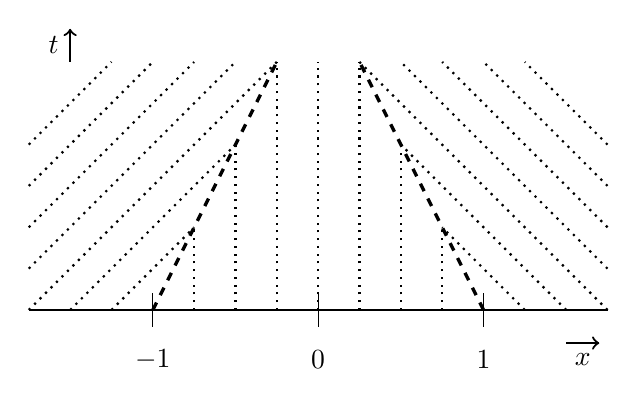
\begin{tikzpicture}[scale=2.1,pile/.style={thick, ->, >=stealth', shorten <=2pt, shorten >=2pt}]

	% Axes
	\draw [-] (-1.75,0) -- (1.75,0);
	\draw[] plot coordinates{ (-1,0.1) (-1,-0.1) };	
	\draw[] plot coordinates{ (0,0.1) (0,-0.1) };	
	\draw[] plot coordinates{ (1,0.1) (1,-0.1) };	
	\draw (-1,-0.3) node { $-1$ };
	\draw (0,-0.3) node { $0$ };
	\draw (1,-0.3) node { $1$ };
	\draw [->,thick] (1.5,-0.2) -- (1.7,-0.2);	
	\draw [->,thick] (-1.5,1.5) -- (-1.5,1.7);		
	\draw (1.6,-0.3) node { $x$ };
	\draw (-1.6,1.6) node { $t$ };

	% Shocks
	\draw [dashed,very thick] (-1,0) -- (-0.25,1.5);
	\draw [dashed,very thick] (1,0) -- (0.25,1.5);
	
	% Straight
	\draw [dotted,thick] (-0.75,0) -- (-0.75,0.5);
	\draw [dotted,thick] (-0.50,0) -- (-0.50,1);
	\draw [dotted,thick] (-0.25,0) -- (-0.25,1.5);
	\draw [dotted,thick] (0,0) -- (0,1.5);
	\draw [dotted,thick] (0.25,0) -- (0.25,1.5);
	\draw [dotted,thick] (0.50,0) -- (0.50,1);
	\draw [dotted,thick] (0.75,0) -- (0.75,0.5);

	% Slopes left
	\draw [dotted,thick] (-1.25,0) -- (-0.75,0.5);
	\draw [dotted,thick] (-1.50,0) -- (-0.50,1);		
	\draw [dotted,thick] (-1.75,0) -- (-0.25,1.5);	
	\draw [dotted,thick] (-1.75,0.25) -- (-0.5,1.5);		
	\draw [dotted,thick] (-1.75,0.50) -- (-0.75,1.5);	
	\draw [dotted,thick] (-1.75,0.75) -- (-1.00,1.5);	
	\draw [dotted,thick] (-1.75,1.00) -- (-1.25,1.5);	
	
	% Slopes right
	\draw [dotted,thick] (1.25,0) -- (0.75,0.5);
	\draw [dotted,thick] (1.50,0) -- (0.50,1);		
	\draw [dotted,thick] (1.75,0) -- (0.25,1.5);	
	\draw [dotted,thick] (1.75,0.25) -- (0.5,1.5);		
	\draw [dotted,thick] (1.75,0.50) -- (0.75,1.5);	
	\draw [dotted,thick] (1.75,0.75) -- (1.00,1.5);	
	\draw [dotted,thick] (1.75,1.00) -- (1.25,1.5);	
			
													
\end{tikzpicture}}
    
    \caption{\label{fig:Exc1_3a} Exercise 3.1a. Initial data $u_0$ given by \label{InCond1}, applied to the inviscid burgers equation. The two shocks move towards each other and merge at $x=0$. At $x=0$ they form a new stationary shock.
    \quad{(a)}~ Initial data. \quad{(b)}~Characteristics. }
    
    \end{figure}
    
    \begin{figure}[H] 
    \center 
    
    \subfloat[\label{fig:Exc1_3b_U}]{\usetikzlibrary{arrows}
\begin{tikzpicture}[scale=2.1,pile/.style={thick, ->, >=stealth', shorten <=2pt, shorten >=2pt}]

	\draw[very thick] plot coordinates{ (-1.75,-1) (-1,-1) (-1,0) (1,0) (1,1) (1.75,1) }; 
	\draw [-] (-1.75,0) -- (1.75,0);
	\draw [dashed] (-1,0) -- (-1.6,-1);
	\draw [dashed] (1,0) -- (1.6,1);
	
	\draw [->,thick] (-1.1,-0.8) -- (-1.4,-0.8);	
	\draw [->,thick] (1.1,0.8) -- (1.4,0.8);	
	
	\draw [->,thick] (-1.5,0.5) -- (-1.5,0.7);	
	\draw [->,thick] (-1.5,0.5) -- (-1.3,0.5);	
	
	\draw (-1.6,0.6) node { $u$ };
	\draw (-1.4,0.4) node { $x$ };
	%\draw (1.25,0.7) node { $u_0(x)$ };

	\draw[ ] plot coordinates{ (0,0.1) (0,-0.1) };	
	\draw (0,-0.3) node { $0$ };


	% Draw fourth fine propagation  
	%\fill[gray!30] (12.5,-3) -- (14,-3) -- (14,-2) -- (12.5,-2) -- (12.5,-3);

	% Draw grid
	%\draw[] plot coordinates{ (0,0) (0,-5) (14,-5) };  
	
	
	
	%\draw [->,very thick] (0,-5.75) -- (2,-5.75);		
	%\draw (1,-5.4) node { $Time$ };

	%\draw [<->,dashed,thick ] (0,1.5) -- (3,1.5);
	%\draw[thick] plot coordinates{ (3,1.4) (3,1.6) };
	
	%\draw (1.5,2) node {$Iter.\,k=0$};	
		
    % Labels
	%\draw (-1.5,0.5) node {$Proc.\,1$};

	% Draw first coarse propagation
	%\fill[gray!90] (0,0) -- (0,1) -- (0.5,1) -- (0.5,0) -- (0,0);
	%\draw[] plot coordinates{ (0,0) (0,1) (0.5,1) (0.5,0) (0,0) };  

	%\draw (13.25,-4.5) node {{\scriptsize $T_{\mathcal{G}}$}};
													
\end{tikzpicture}
%
%\draw plot coordinates{point sequence};	
%\draw plot ;	
%	\draw[smooth] plot coordinates{(0,0),{};
% \draw [smooth,very thick] (0,0) -- (4,-3) -- (8,-5) -- (12,-6);
% \draw[smooth,domain=0:6.5] plot function{sin(2*x)*exp(-x/4)};
% \draw[ycomb,color=gray,line width=0.5cm] plot coordinates{(1,1) (2,2) (3,3)};
}
    \hspace{10mm}
    \subfloat[\label{fig:Exc1_3b_C}]{\usetikzlibrary{arrows}
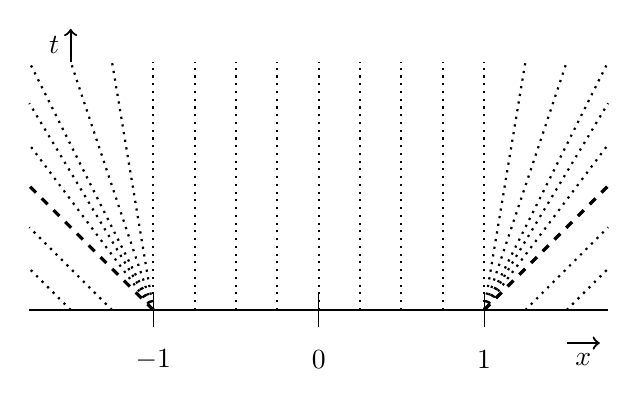
\begin{tikzpicture}[scale=2.1,pile/.style={thick, ->, >=stealth', shorten <=2pt, shorten >=2pt}]

	% Axes
	\draw [-] (-1.75,0) -- (1.75,0);
	\draw[] plot coordinates{ (-1,0.1) (-1,-0.1) };	
	\draw[] plot coordinates{ (0,0.1) (0,-0.1) };	
	\draw[] plot coordinates{ (1,0.1) (1,-0.1) };	
	\draw (-1,-0.3) node { $-1$ };
	\draw (0,-0.3) node { $0$ };
	\draw (1,-0.3) node { $1$ };
	\draw [->,thick] (1.5,-0.2) -- (1.7,-0.2);	
	\draw [->,thick] (-1.5,1.5) -- (-1.5,1.7);		
	\draw (1.6,-0.3) node { $x$ };
	\draw (-1.6,1.6) node { $t$ };
	
	% Straight
	\draw [dotted,thick] (-1,0) -- (-1,1.5);
	\draw [dotted,thick] (-0.75,0) -- (-0.75,1.5);
	\draw [dotted,thick] (-0.5,0) -- (-0.5,1.5);
	\draw [dotted,thick] (-0.25,0) -- (-0.25,1.5);
	\draw [dotted,thick] (0,0) -- (0,1.5);
	\draw [dotted,thick] (0.25,0) -- (0.25,1.5);
	\draw [dotted,thick] (0.5,0) -- (0.5,1.5);	
	\draw [dotted,thick] (0.75,0) -- (0.75,1.5);	
	\draw [dotted,thick] (1,0) -- (1,1.5);


	% Slopes left
	\draw [dotted,thick] (-1.5,0) -- (-1.75,0.25);
	\draw [dotted,thick] (-1.25,0) -- (-1.75,0.50);
	\draw [dashed, very thick] (-1,0) -- (-1.75,0.75);
	\draw [dotted,thick] (-1,0) -- (-1.75,1);
	\draw [dotted,thick] (-1,0) -- (-1.75,1.25);
	\draw [dotted,thick] (-1,0) -- (-1.75,1.50);
	\draw [dotted,thick] (-1,0) -- (-1.50,1.50);
	\draw [dotted,thick] (-1,0) -- (-1.25,1.50);
				
	% Slopes right
	\draw [dotted,thick] (1.5,0) -- (1.75,0.25);
	\draw [dotted,thick] (1.25,0) -- (1.75,0.50);
	\draw [dashed,very thick] (1,0) -- (1.75,0.75);
	\draw [dotted,thick] (1,0) -- (1.75,1);
	\draw [dotted,thick] (1,0) -- (1.75,1.25);
	\draw [dotted,thick] (1,0) -- (1.75,1.50);
	\draw [dotted,thick] (1,0) -- (1.50,1.50);
	\draw [dotted,thick] (1,0) -- (1.25,1.50);			
													
\end{tikzpicture}
}
    
    \caption{\label{fig:Exc1_3b} Exercise 3.1b. Initial data $u_0$, given by \label{InCond2}, applied to the inviscid burgers equation. The two rarefaction waves move away from each other with equal speed and never merge. \quad{(a)} Initial data. \quad{(b)} Characteristics. }
    
    \end{figure}
    
    \begin{figure}[H]
    \center 
    
    \subfloat[\label{fig:Exc1_4_U}]{\usetikzlibrary{arrows}
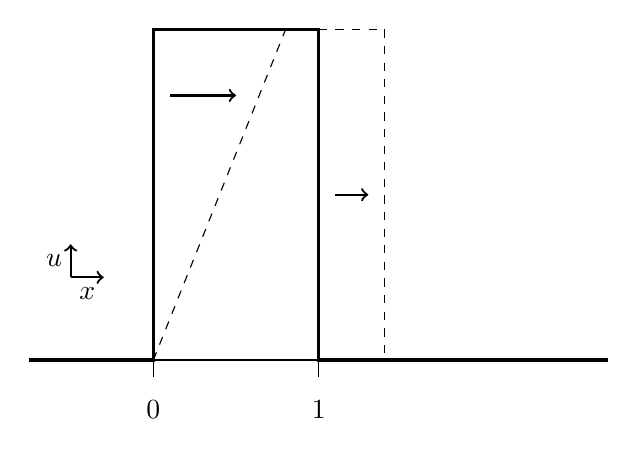
\begin{tikzpicture}[scale=2.1,pile/.style={thick, ->, >=stealth', shorten <=2pt, shorten >=2pt}]

	\draw[very thick] plot coordinates{ (-0.75,0) (0,0) (0,2) (1,2) (1,0) (2.75,0) }; 
	\draw [-] (-0.75,0) -- (2.75,0);
	\draw [dashed] (0,0) -- (0.8,2);
	\draw [dashed] (0.8,2) -- (1.4,2);
	\draw [dashed] (1.4,2) -- (1.4,0);
	
	\draw [->,thick] (-0.5,0.5) -- (-0.5,0.7);	
	\draw [->,thick] (-0.5,0.5) -- (-0.3,0.5);	

	
	\draw [->,thick] (0.1,1.6) -- (0.5,1.6);		
	\draw [->,thick] (1.1,1) -- (1.3,1);	
	
	\draw (-0.6,0.6) node { $u$ };
	\draw (-0.4,0.4) node { $x$ };

	\draw[] plot coordinates{ (0,0.1) (0,-0.1) };	
	\draw[] plot coordinates{ (1,0.1) (1,-0.1) };	
	\draw (0,-0.3) node { $0$ };
	\draw (1,-0.3) node { $1$ };

	%\draw (2.25,0.7) node { $u_0(x)$ };

	% Draw fourth fine propagation  
	%\fill[gray!30] (12.5,-3) -- (14,-3) -- (14,-2) -- (12.5,-2) -- (12.5,-3);

	% Draw grid
	%\draw[] plot coordinates{ (0,0) (0,-5) (14,-5) };  
	
	
	
	%\draw [->,very thick] (0,-5.75) -- (2,-5.75);		
	%\draw (1,-5.4) node { $Time$ };

	%\draw [<->,dashed,thick ] (0,1.5) -- (3,1.5);
	%\draw[thick] plot coordinates{ (3,1.4) (3,1.6) };
	
	%\draw (1.5,2) node {$Iter.\,k=0$};	
		
    % Labels
	%\draw (-1.5,0.5) node {$Proc.\,1$};

	% Draw first coarse propagation
	%\fill[gray!90] (0,0) -- (0,1) -- (0.5,1) -- (0.5,0) -- (0,0);
	%\draw[] plot coordinates{ (0,0) (0,1) (0.5,1) (0.5,0) (0,0) };  

	%\draw (13.25,-4.5) node {{\scriptsize $T_{\mathcal{G}}$}};
													
\end{tikzpicture}
%
%\draw plot coordinates{point sequence};	
%\draw plot ;	
%	\draw[smooth] plot coordinates{(0,0),{};
% \draw [smooth,very thick] (0,0) -- (4,-3) -- (8,-5) -- (12,-6);
% \draw[smooth,domain=0:6.5] plot function{sin(2*x)*exp(-x/4)};
% \draw[ycomb,color=gray,line width=0.5cm] plot coordinates{(1,1) (2,2) (3,3)};
}
    \hspace{10mm}
    \subfloat[\label{fig:Exc1_4_C}]{\usetikzlibrary{arrows}
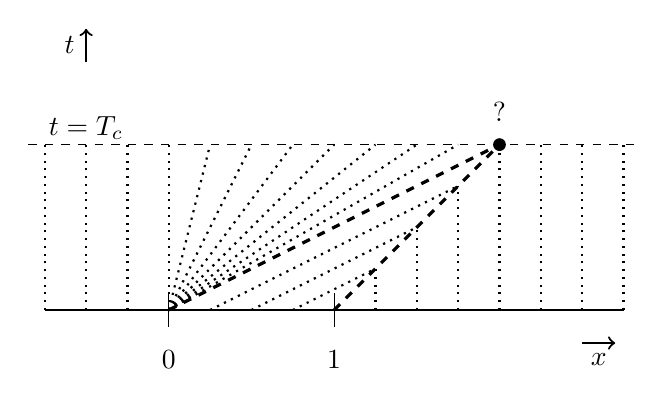
\begin{tikzpicture}[scale=2.1,pile/.style={thick, ->, >=stealth', shorten <=2pt, shorten >=2pt}]

	\draw [-] (-0.75,0) -- (2.75,0);
	\draw [dashed, very thick] (1,0) -- (2,1);
	

	% Straight
	\draw [dotted,thick] (-0.75,0) -- (-0.75,1.00);
	\draw [dotted,thick] (-0.50,0) -- (-0.50,1.00);
	\draw [dotted,thick] (-0.25,0) -- (-0.25,1.00);
	\draw [dotted,thick] (-0.0,0) -- (-0.0,1.00);		
	\draw [dotted,thick] (1.25,0) -- (1.25,0.25);
	\draw [dotted,thick] (1.50,0) -- (1.50,0.50);
	\draw [dotted,thick] (1.75,0) -- (1.75,0.75);
	\draw [dotted,thick] (2.00,0) -- (2.00,1.00);	
	\draw [dotted,thick] (2.25,0) -- (2.25,1.00);	
	\draw [dotted,thick] (2.50,0) -- (2.50,1.00);
	\draw [dotted,thick] (2.75,0) -- (2.75,1.00);	
	
	% Within Rarefaction
	\draw [dashed,very thick] (0,0) -- (2,1.00);
	\draw [dotted,thick] (0.25,0) -- (1.75,0.75);
	\draw [dotted,thick] (0.5,0) -- (1.5,0.5);
	\draw [dotted,thick] (0.75,0) -- (1.25,0.25);
	
	\draw [dotted,thick] (0,0) -- (0.25,1.00);
	\draw [dotted,thick] (0,0) -- (0.50,1.00);
	\draw [dotted,thick] (0,0) -- (0.75,1.00);
	\draw [dotted,thick] (0,0) -- (1.00,1.00);	
	\draw [dotted,thick] (0,0) -- (1.25,1.00);
	\draw [dotted,thick] (0,0) -- (1.50,1.00);		
	\draw [dotted,thick] (0,0) -- (1.75,1.00);	
				
	\draw[] plot coordinates{ (0,0.1) (0,-0.1) };	
	\draw[] plot coordinates{ (1,0.1) (1,-0.1) };	
	\draw (0,-0.3) node { $0$ };
	\draw (1,-0.3) node { $1$ };
	
	\draw [->,thick] (2.5,-0.2) -- (2.7,-0.2);	
	\draw [->,thick] (-0.5,1.5) -- (-0.5,1.7);		
	\draw (2.6,-0.3) node { $x$ };
	\draw (-0.6,1.6) node { $t$ };

	% Question
	\draw [dashed] (-0.85,1) -- (2.85,1);	
	\draw (-0.5,1.1) node { $t=T_c$ };
	\draw (2,1.2) node { $?$ };
	\filldraw (2,1) circle (1pt);
	
	% Draw fourth fine propagation  
	%\fill[gray!30] (12.5,-3) -- (14,-3) -- (14,-2) -- (12.5,-2) -- (12.5,-3);

	% Draw grid
	%\draw[] plot coordinates{ (0,0) (0,-5) (14,-5) };  
	
	
	
	%\draw [->,very thick] (0,-5.75) -- (2,-5.75);		
	%\draw (1,-5.4) node { $Time$ };

	%\draw [<->,dashed,thick ] (0,1.5) -- (3,1.5);
	%\draw[thick] plot coordinates{ (3,1.4) (3,1.6) };
	
	%\draw (1.5,2) node {$Iter.\,k=0$};	
		
    % Labels
	%\draw (-1.5,0.5) node {$Proc.\,1$};

	% Draw first coarse propagation
	%\fill[gray!90] (0,0) -- (0,1) -- (0.5,1) -- (0.5,0) -- (0,0);
	%\draw[] plot coordinates{ (0,0) (0,1) (0.5,1) (0.5,0) (0,0) };  

	%\draw (13.25,-4.5) node {{\scriptsize $T_{\mathcal{G}}$}};
													
\end{tikzpicture}
%
%\draw plot coordinates{point sequence};	
%\draw plot ;	
%	\draw[smooth] plot coordinates{(0,0),{};
% \draw [smooth,very thick] (0,0) -- (4,-3) -- (8,-5) -- (12,-6);
% \draw[smooth,domain=0:6.5] plot function{sin(2*x)*exp(-x/4)};
% \draw[ycomb,color=gray,line width=0.5cm] plot coordinates{(1,1) (2,2) (3,3)};
}
    
    \caption{\label{fig:Exc1_4} Exercise 3.2. Initial data $u_0$, given by \label{inCond3}, applied to the inviscid burgers equation. The rarefaction wave and the shock both move in the positive direction. The rarefaction wave moves faster than the shock and at some point in time $t=T_c>0$ they meet. \quad{(a)} Initial data. \quad{(b)} Characteristics. }
    \end{figure}
\end{solution}


























\bibliography{ref}{}
\bibliographystyle{plain}
\end{document}
